%Written with Anthony Savagar (https://github.com/asavagar)
%adapted from https://tex.stackexchange.com/questions/78846/creating-thicker-tikz-mindmap-connectors
\documentclass[10pt,margin=5pt]{standalone}
\usepackage{tikz}
\renewcommand*\familydefault{\sfdefault}
\usetikzlibrary{mindmap,trees,shadows}

\begin{document}

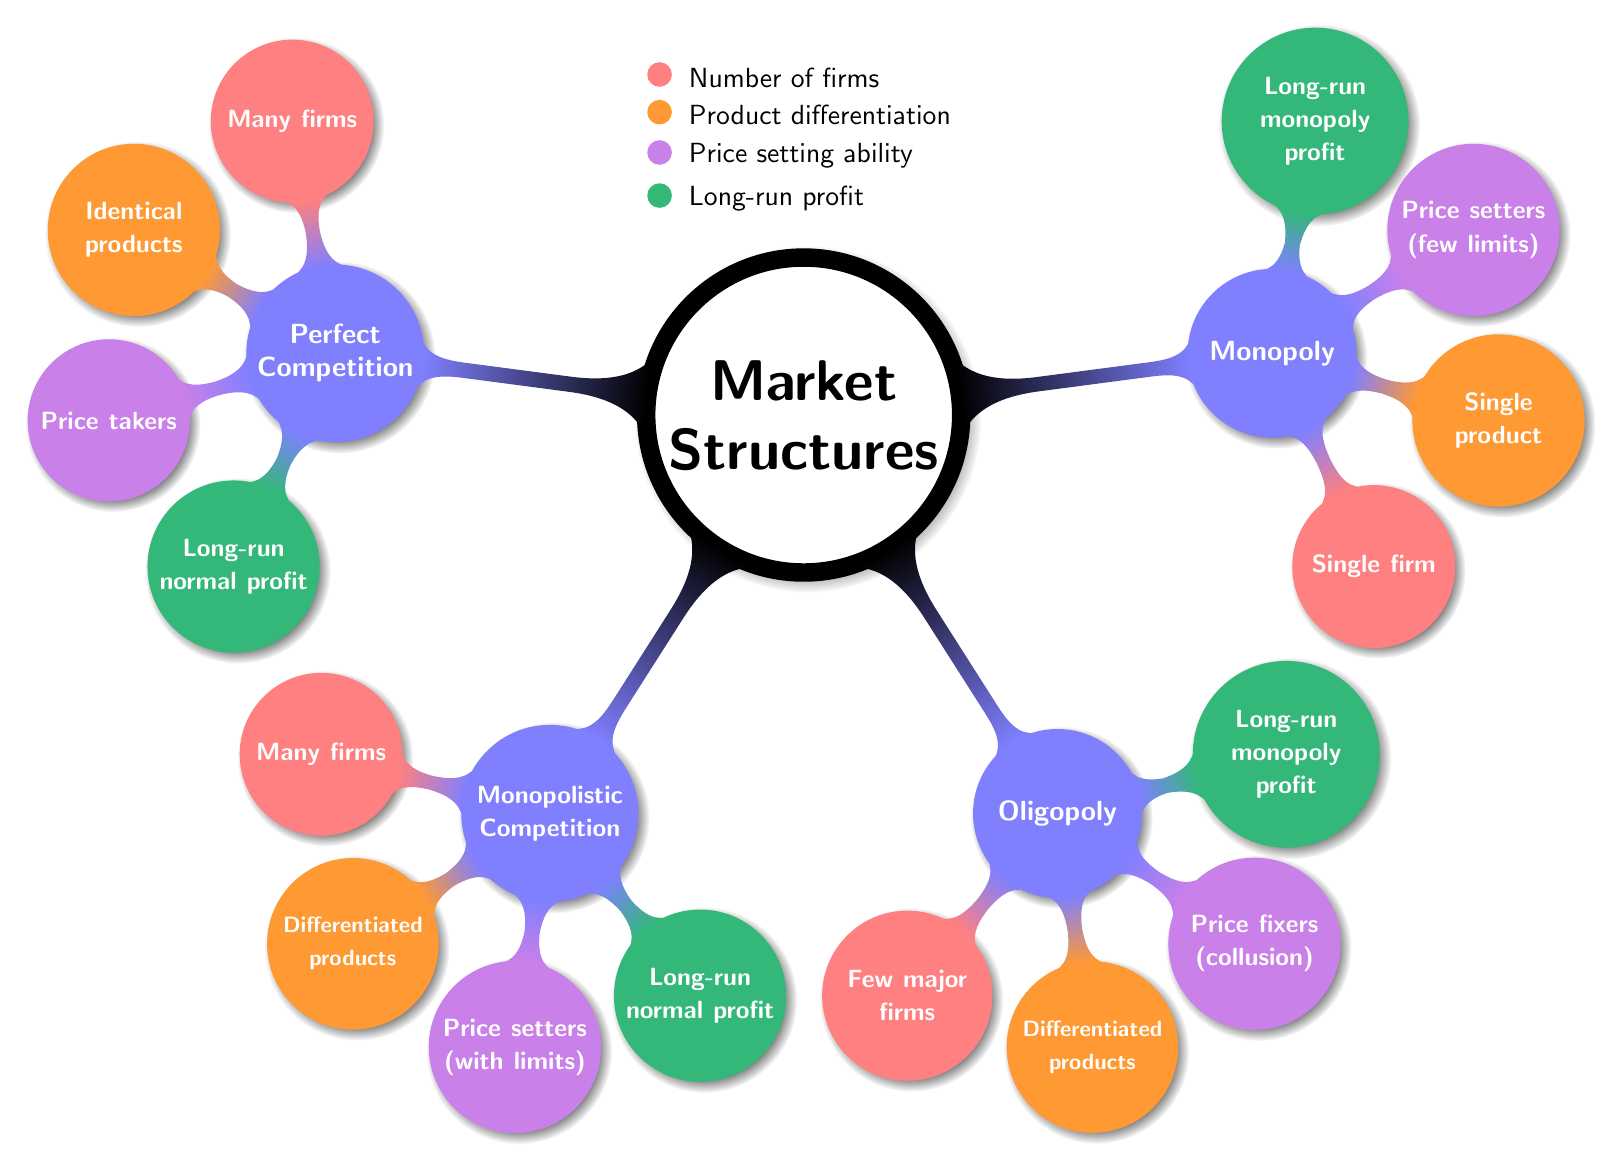
\begin{tikzpicture}[decoration={start radius=1cm, end radius=.5cm,amplitude=3mm,angle=30}]

% Define experience colors
\definecolor{codepurple}{rgb}{0.58,0,0.82}
\colorlet{firmcolor}{red!50}
\colorlet{productcolor}{orange!80}
\colorlet{pricecolor}{codepurple!50}
\colorlet{profitcolor}{teal!70!green!80}
\colorlet{sparecolor}{violet!75}

\begin{scope}[mindmap,
every node/.style={concept, circular drop shadow, minimum size=0pt,execute at begin node=\hskip0pt, font=\bfseries},
root concept/.append style={
    concept color=black, fill=white, line width=1.5ex, text=black, font=\huge\scshape\bfseries,},
level 1 concept/.append style={font=\bfseries},
text=white,
market/.style={concept color=blue!50},
firms/.style={concept color=firmcolor},
product/.style={concept color=productcolor},
power/.style={concept color=pricecolor},
profit/.style={concept color=profitcolor},
cits/.style={concept color=sparecolor},
grow cyclic,
level 1/.append style={level distance=6cm,sibling angle=65}, %Use to alter gaps between the main nodes
level 2/.append style={level distance=3cm,sibling angle=48,minimum size=5.5em,text width=5.5em}] %Use to alter gaps between the smaller nodes and affect the size of these nodes
\node [root concept] (team) {Market\\Structures}[rotate=-90] %rotate the placement of the main nodes
    child [market] { node {Perfect Competition}
        child [firms] { node {\small Many firms} }
        child [product] { node {\small Identical products} }
        child [power] { node {\small Price takers} }
        child [profit] { node {\small Long-run normal profit} }
    }
    child [market] { node {\small Monopolistic Competition}
        child [firms] { node {\small Many firms} }
    	child [product] { node {\footnotesize Differentiated products} }
    	child [power] { node {\small Price setters (with limits)} }
    	child [profit] { node {\small Long-run normal profit} }
    }
    child [market] { node (comp3) {Oligopoly}
        child [firms] { node {\small Few major firms} }
        child [product] { node {\footnotesize Differentiated products} }
        child [power] { node {\small Price fixers (collusion)} }
        child [profit] { node {\small Long-run monopoly profit} }
    }
    child [market] { node {Monopoly}
        child [firms] { node {\small Single firm} }
        child [product] { node {\small Single product} }
        child [power] { node {\small Price setters (few limits)} }
        child [profit] { node {\small Long-run monopoly profit} }
    }
    ;
\end{scope}

\begin{scope}[xshift=0cm, yshift=3.5cm,every node/.style={align=left,text=black}]
\matrix[row sep=0pt,column sep=1mm, align=left, nodes={align=left, anchor=west}] {
    \fill [firmcolor] (0,.25ex) circle (1ex); & \node{Number of firms};\\
    \fill [productcolor] (0,.25ex) circle (1ex); & \node{Product differentiation};\\
    \fill [pricecolor] (0,.25ex) circle (1ex); & \node{Price setting ability};\\
    \fill [profitcolor] (0,.25ex) circle (1ex); & \node{Long-run profit};\\
    };
\end{scope}
\end{tikzpicture}

\end{document}